\documentclass[11pt]{article}
\usepackage[margin=1in]{geometry}
\usepackage{graphicx}
\usepackage{booktabs}
\usepackage{amsmath}
\usepackage{hyperref}
\usepackage{float}
\usepackage{enumitem}
\usepackage{caption}
\usepackage{subcaption}
\usepackage{multirow}

\setlength{\parskip}{6pt}
\setlength{\parindent}{0pt}

\begin{document}
\begin{titlepage}
	\clearpage\thispagestyle{empty}
	\centering
	\vspace{1cm}

	\rule{\linewidth}{1mm} \\[0.5cm]
	{ \Large \bfseries ISyE 6740 --- Spring 2026\\[0.2cm]
		Final Project Report}\\[0.5cm]
	\rule{\linewidth}{1mm} \\[1cm]

		\begin{tabular}{l p{8cm}}
		\textbf{Team Member Names:} & Pramodh Aryasomayajula, Keshav Shah \\[10pt]
		\textbf{Project Title:} & Predicting Environmental Compliance Violations at Small Manufacturing Facilities Using EPA ECHO Data \\[10pt]
		\end{tabular}

	\pagebreak

\end{titlepage}


%% ============================================================
\section{Problem Statement}
%% ============================================================

The U.S. Environmental Protection Agency (EPA) regulates approximately 800,000 facilities under statutes including the Clean Air Act (CAA), Clean Water Act (CWA), and Resource Conservation and Recovery Act (RCRA). However, regulatory agencies are resource-constrained, and smaller facilities often receive less oversight than those classified as ``major sources.'' Small manufacturers---establishments in NAICS sectors 31--33 with non-major regulatory designations---represent a substantial share of the regulated population. For these firms, compliance is highly burdensome, costing over \$50,000 per employee annually \cite{nam2023}.

This project asks: \textit{can we predict which small manufacturing facilities will experience environmental compliance violations in the next year, using only historical compliance patterns and facility characteristics?} A reliable predictive model would help regulators prioritize inspections and help manufacturers understand which traits correlate with non-compliance.

We frame this as a binary classification task. Using the EPA's Enforcement and Compliance History Online (ECHO) database, we construct a pseudo-temporal prediction problem by splitting each facility's 12-quarter compliance history string into a 2-year feature window and a 1-year target window. We compare four classifiers---Logistic Regression, Random Forest, XGBoost, and SVM---and evaluate them using AUC-ROC, AUC-PR, and bootstrap confidence intervals. To our knowledge, supervised learning has not been applied to the small manufacturer segment of ECHO data for violation prediction.


%% ============================================================
\section{Data Description and Cleaning}
%% ============================================================

\subsection{Data Source}

Our dataset comes from the EPA ECHO Exporter, a weekly-updated bulk download containing facility-level summaries for all regulated establishments in the United States. The export file contains 3,091,085 facilities across 133 columns, covering facility identification, geographic location, regulatory program participation, inspection and enforcement history, penalty amounts, and quarterly compliance status.

\subsection{Population Filtering}

We applied the following filters to isolate our target population:
\begin{enumerate}
    \item \textbf{Industry}: Retained facilities whose NAICS codes include at least one manufacturing sector code (31, 32, or 33).
    \item \textbf{Size proxy}: Excluded facilities flagged as ``major'' (\texttt{FAC\_MAJOR\_FLAG = Y}), using non-major status as a proxy for smaller establishments.
    \item \textbf{Activity}: Retained only active facilities (\texttt{FAC\_ACTIVE\_FLAG = Y}).
    \item \textbf{History completeness}: Required a full 12-quarter compliance history string.
\end{enumerate}

After filtering, our final dataset contains approximately 120,000 small manufacturing facilities.

\subsection{Target Variable Construction}

The ECHO Exporter includes a field \texttt{FAC\_3YR\_COMPLIANCE\_HISTORY}, a 12-character string where each character encodes one quarter's compliance status over the past three years. Characters include \texttt{\_} (no violation), \texttt{V} (violation), \texttt{S} (significant non-compliance), and \texttt{U} (unknown). Position 0 is the oldest quarter and position 11 is the most recent.

We split this string to create a pseudo-temporal prediction problem:
\begin{itemize}
    \item \textbf{Feature window} (positions 0--7): the older 2 years, used to derive predictive features.
    \item \textbf{Target window} (positions 8--11): the most recent 1 year. The binary target is 1 if any character in this window is \texttt{V} or \texttt{S}, and 0 otherwise.
\end{itemize}

This design simulates the real-world task of predicting next-year violations from historical data, even though the underlying dataset is a cross-sectional snapshot. The resulting positive class rate is approximately 8.1\%, confirming the moderate class imbalance anticipated in our proposal.

\subsection{Feature Engineering}

We engineered features across four categories:

\begin{table}[H]
\centering
\caption{Feature categories and descriptions}
\small
\begin{tabular}{p{3.2cm} p{4cm} p{5cm}}
\toprule
\textbf{Category} & \textbf{Features} & \textbf{Description} \\
\midrule
Compliance History & \texttt{n\_nc\_qtrs}, \texttt{n\_snc\_qtrs}, \texttt{violation\_trend}, \texttt{last\_nc\_distance}, \texttt{longest\_clean\_streak}, \texttt{recency\_weighted} & Derived from the 8-quarter feature window of the general, CAA, CWA, and RCRA history strings \\
\addlinespace
Industry & \texttt{naics\_2digit}, \texttt{naics\_3digit} & Parsed from the primary manufacturing NAICS code \\
\addlinespace
Geography \& Demographics & \texttt{fac\_state}, \texttt{fac\_epa\_region}, \texttt{fac\_lat}, \texttt{fac\_long}, \texttt{percent\_minority}, \texttt{pop\_den} & State, EPA region, coordinates, and census demographics \\
\addlinespace
Regulatory Profile & Program flags (CAA, CWA, RCRA, SDWA, TRI, GHG), \texttt{n\_programs}, inspection counts, penalty counts & Number and type of regulatory programs, historical inspection and enforcement activity \\
\bottomrule
\end{tabular}
\end{table}

\subsection{Data Leakage Prevention}

Several ECHO fields directly encode the full 12-quarter compliance history or current status and would leak the target variable. We excluded: \texttt{FAC\_QTRS\_WITH\_NC} (exactly equals the count of V/S across all 12 quarters), \texttt{FAC\_COMPLIANCE\_STATUS}, \texttt{FAC\_SNC\_FLG}, all program-specific \texttt{*\_COMPLIANCE\_STATUS} and \texttt{*\_SNC\_FLAG} fields, and \texttt{FAC\_DAYS\_LAST\_INSPECTION}. Cumulative lifetime counts (e.g., \texttt{FAC\_INSPECTION\_COUNT}) were retained but subjected to a sensitivity analysis to quantify any soft leakage from including target-period activity in these totals.


%% ============================================================
\section{Methodology}
%% ============================================================

\subsection{Preprocessing}

We applied median imputation for the small number of missing values in \texttt{FAC\_PERCENT\_MINORITY} and \texttt{FAC\_POP\_DEN}, and filled program-specific counts with zero where the facility does not participate in that program. Categorical features with high cardinality (\texttt{naics\_3digit} with $\sim$80 categories, \texttt{fac\_state} with $\sim$50) were target-encoded using scikit-learn's \texttt{TargetEncoder} with internal cross-fitting to prevent leakage during cross-validation. Low-cardinality categoricals (\texttt{naics\_2digit}, \texttt{fac\_epa\_region}) were one-hot encoded. All numeric features were standardized with \texttt{StandardScaler}. The full pipeline was implemented using \texttt{ColumnTransformer} to ensure all transformations are fit only on training data.

Data was split 80/20 into training and test sets with stratification by the target variable.

\subsection{Models}

We trained four classifiers, chosen to span a range of complexity and interpretability:

\textbf{Logistic Regression (L1).} Our interpretable baseline. The L1 (Lasso) penalty performs embedded feature selection by driving less predictive coefficients to zero. We tuned the regularization parameter $C \in \{0.001, 0.01, 0.1, 1, 10\}$ using 5-fold stratified cross-validation with AUC-ROC as the scoring metric. Class weights were set to ``balanced'' to account for imbalance.

\textbf{Random Forest.} An ensemble of decision trees that handles mixed feature types well and provides built-in feature importance. We tuned the number of trees $\{200, 500\}$, maximum depth $\{5, 10, 20\}$, and minimum samples per leaf $\{5, 20, 50\}$ via grid search with balanced class weights.

\textbf{XGBoost.} A gradient-boosted tree model that typically achieves state-of-the-art performance on tabular data \cite{chen2016}. We used \texttt{scale\_pos\_weight} to address imbalance and tuned depth, learning rate, number of estimators, subsample ratio, and column sample ratio using randomized search (30 configurations).

\textbf{SVM (RBF Kernel).} Included to test whether a non-linear kernel-based boundary improves classification. Due to the $O(n^2)$ memory complexity of the kernel matrix, we trained on a stratified subsample of 12,000 rows and evaluated on the full test set. We tuned $C \in \{0.1, 1, 10\}$ and $\gamma \in \{\text{scale}, 0.01, 0.001\}$.

\subsection{Class Imbalance Handling}

Given the $\sim$8\% positive class rate, we compared three strategies using the best XGBoost configuration: (1) no weighting, (2) class weighting via \texttt{scale\_pos\_weight}, and (3) SMOTE oversampling applied inside the cross-validation loop using \texttt{imblearn.pipeline.Pipeline} to prevent information leakage from the test folds.


%% ============================================================
\section{Results and Evaluation}
%% ============================================================

\subsection{Model Comparison}

All models were evaluated on the held-out test set. We report AUC-ROC with 95\% bootstrap confidence intervals (1,000 resamples), AUC-PR (average precision), and precision/recall/F1 at the threshold maximizing Youden's J statistic.

\begin{table}[H]
\centering
\caption{Model performance on held-out test set. Confidence intervals are 95\% bootstrap.}
\small
\begin{tabular}{lccccc}
\toprule
\textbf{Model} & \textbf{AUC-ROC [95\% CI]} & \textbf{AUC-PR} & \textbf{Precision} & \textbf{Recall} & \textbf{F1} \\
\midrule
Logistic Regression & 0.960 [0.956, 0.963] & 0.733 & 0.380 & 0.910 & 0.536 \\
Random Forest       & \textbf{0.974} [0.972, 0.977] & \textbf{0.827} & 0.471 & 0.922 & \textbf{0.623} \\
XGBoost             & 0.974 [0.971, 0.977] & 0.827 & 0.463 & 0.917 & 0.616 \\
SVM (RBF)           & 0.957 [0.953, 0.961] & 0.698 & 0.414 & 0.903 & 0.567 \\
\bottomrule
\end{tabular}
\label{tab:results}
\end{table}

\begin{figure}[H]
    \centering
    \begin{subfigure}[b]{0.48\textwidth}
        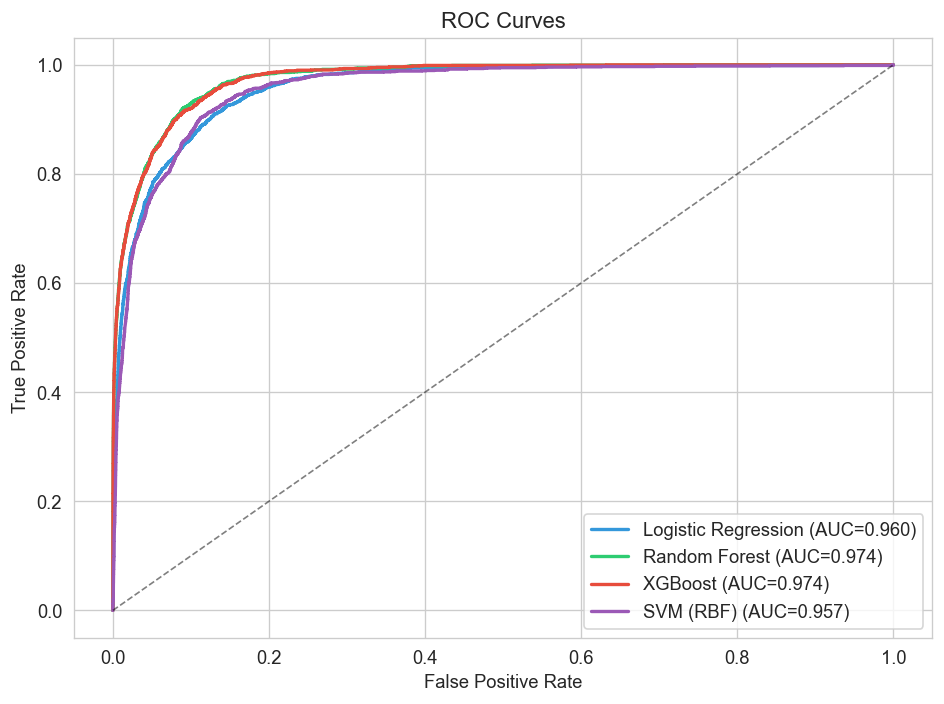
\includegraphics[width=\textwidth]{figures/roc_curves.png}
        \caption{ROC curves}
    \end{subfigure}
    \hfill
    \begin{subfigure}[b]{0.48\textwidth}
        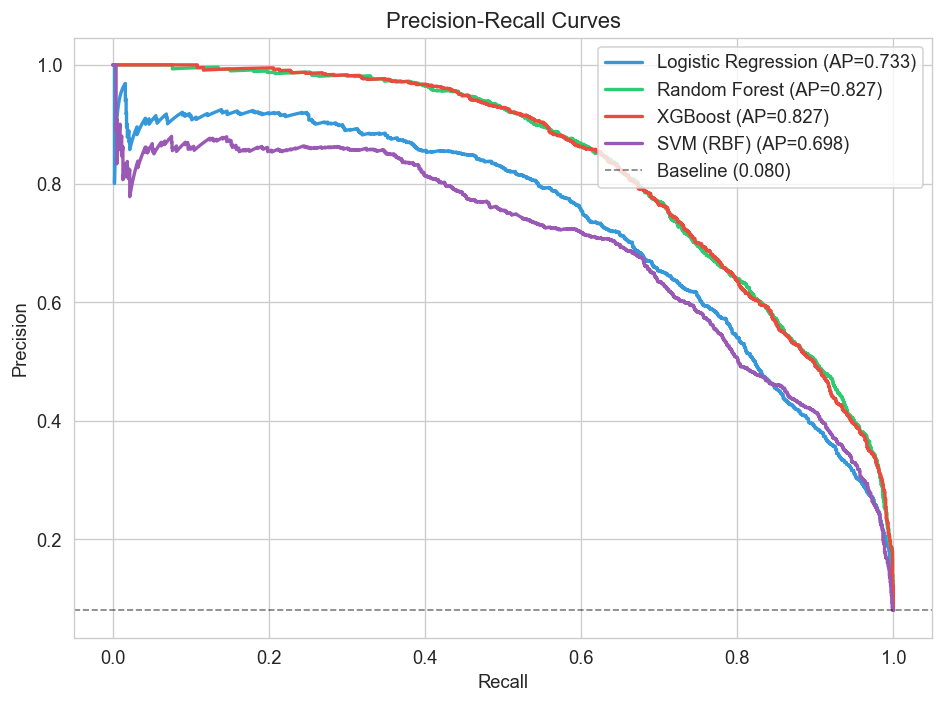
\includegraphics[width=\textwidth]{figures/pr_curves.png}
        \caption{Precision-Recall curves}
    \end{subfigure}
    \caption{Discrimination performance across all four models. The dashed line in (a) represents random classification; in (b), it represents the baseline positive class rate.}
    \label{fig:curves}
\end{figure}

\begin{figure}[H]
    \centering
    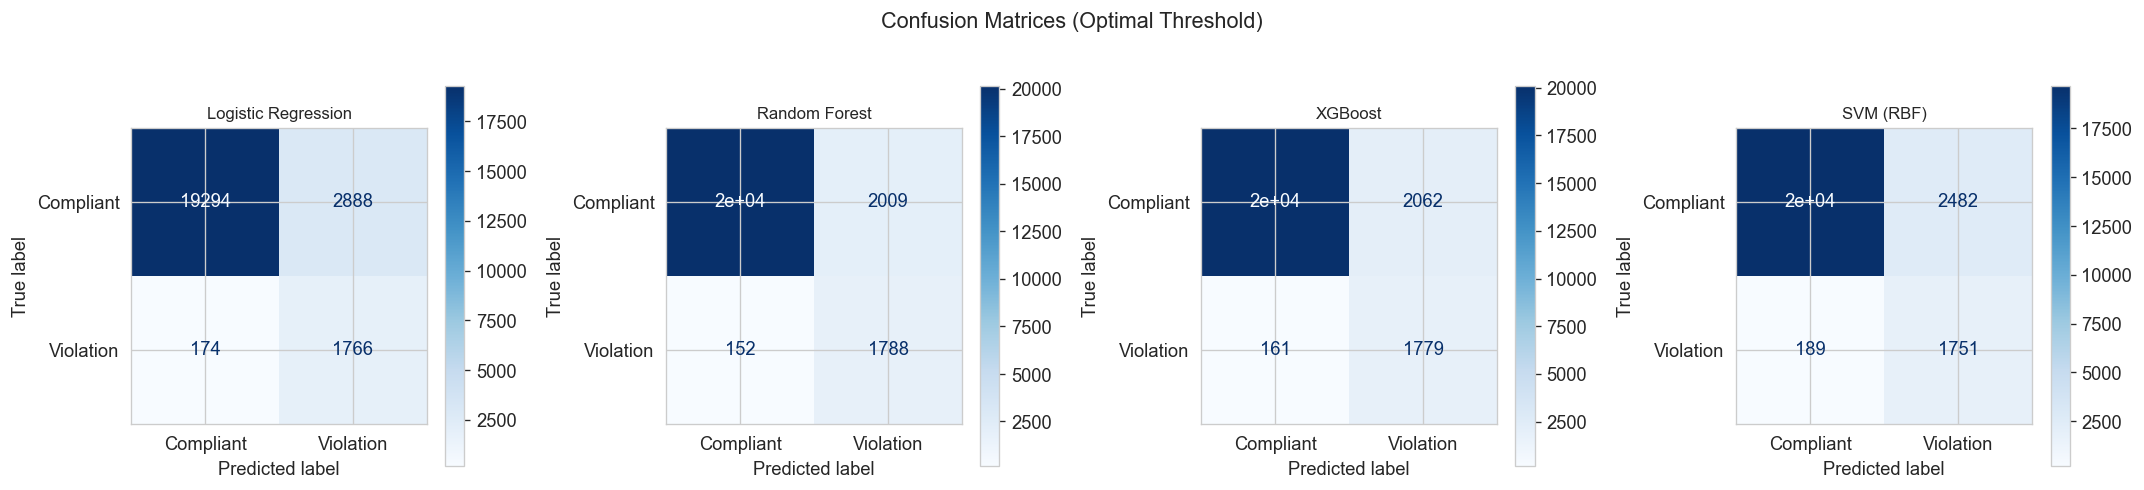
\includegraphics[width=0.95\textwidth]{figures/confusion_matrices.png}
    \caption{Confusion matrices at the optimal threshold (Youden's J) for each model.}
    \label{fig:cm}
\end{figure}

\subsection{Feature Importance}

We compared feature importance across three models to identify which facility traits are most predictive of violations:

\begin{figure}[H]
    \centering
    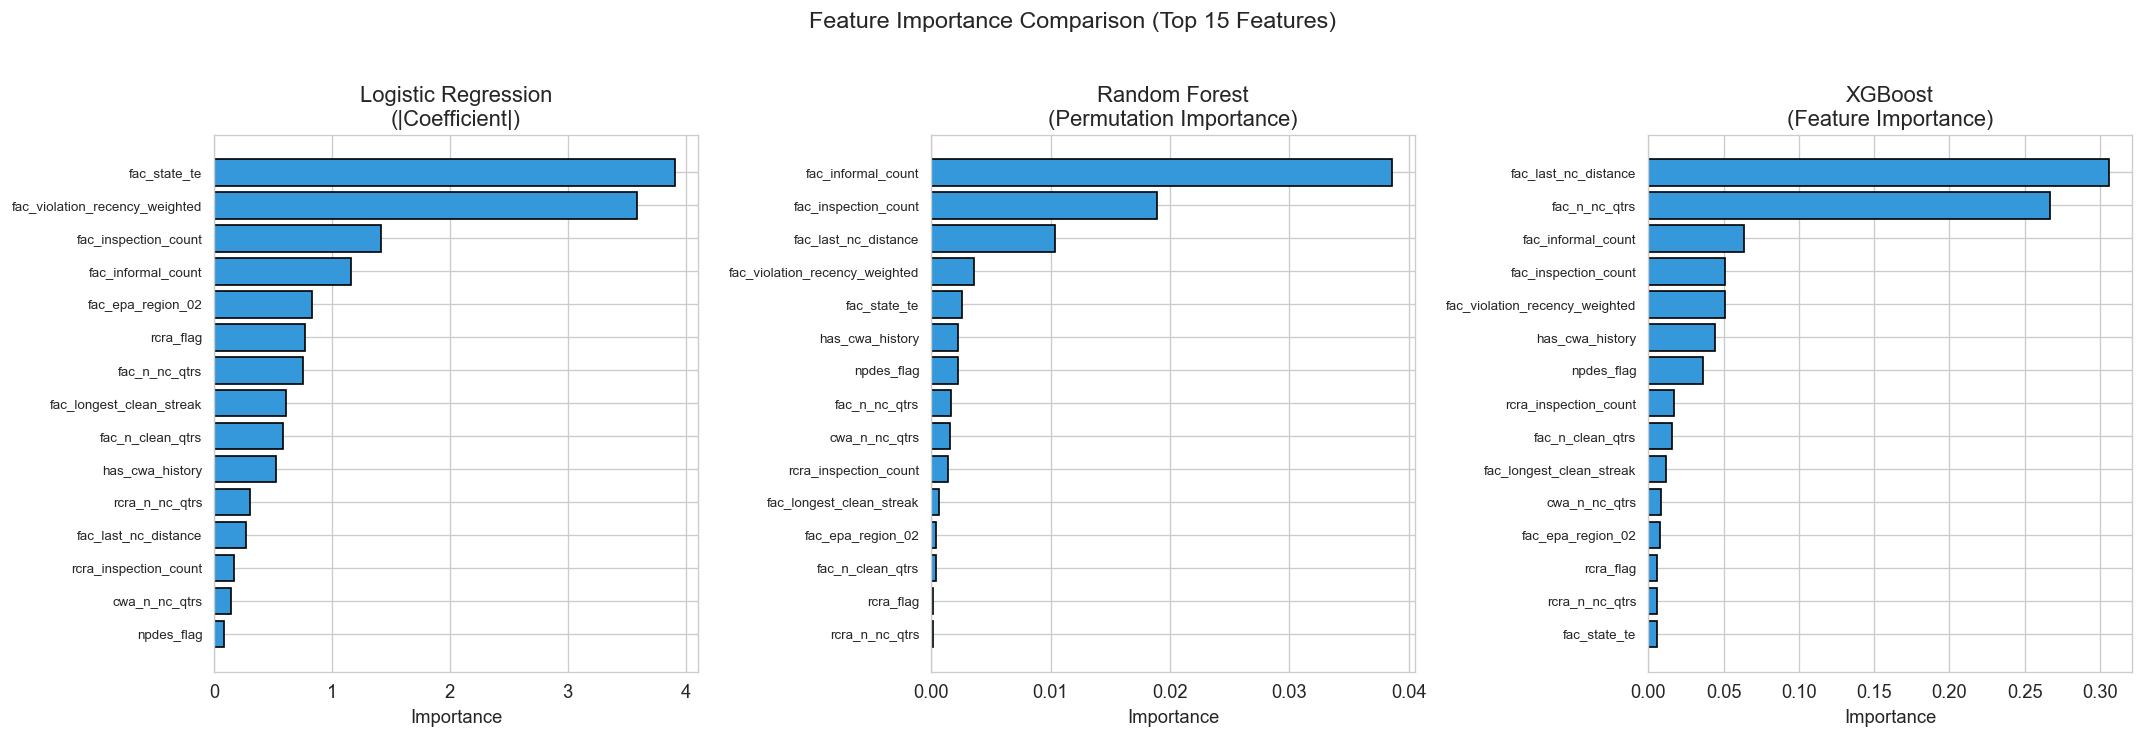
\includegraphics[width=0.95\textwidth]{figures/feature_importance.png}
    \caption{Feature importance comparison. Logistic Regression uses absolute coefficient magnitude, Random Forest uses permutation importance, and XGBoost uses built-in gain-based importance.}
    \label{fig:importance}
\end{figure}

\begin{figure}[H]
    \centering
    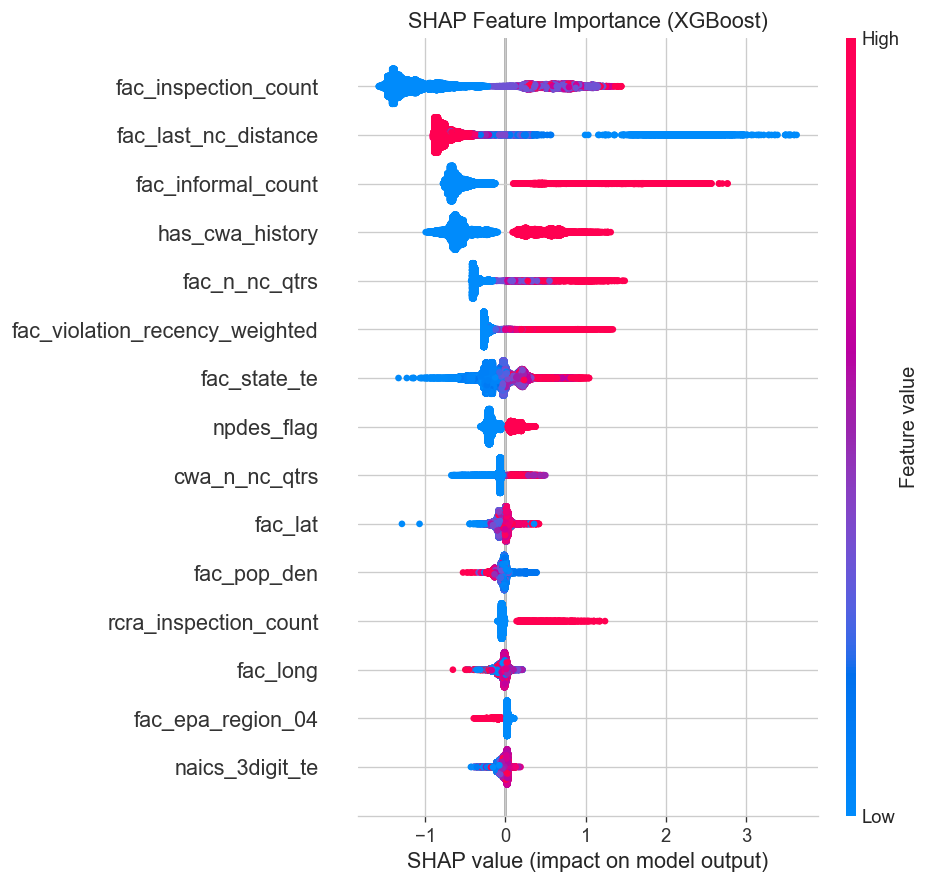
\includegraphics[width=0.75\textwidth]{figures/shap_beeswarm.png}
    \caption{SHAP beeswarm plot for the XGBoost model showing the direction and magnitude of each feature's impact on predictions.}
    \label{fig:shap}
\end{figure}

Across all three models, the strongest predictors are compliance history features: the number of non-compliant quarters in the feature window, recency-weighted violation score, and the distance since the last non-compliance event. This aligns with the environmental compliance literature, which finds that past violations are the strongest predictor of future violations. The number of active regulatory programs also appears among the top features, likely because facilities subject to more programs have more opportunities for violations to be detected.

\subsection{Class Imbalance Experiments}

\begin{table}[H]
\centering
\caption{Class imbalance strategy comparison (XGBoost)}
\begin{tabular}{lcc}
\toprule
\textbf{Strategy} & \textbf{AUC-ROC} & \textbf{AUC-PR} \\
\midrule
No Weighting    & \textbf{0.974} & \textbf{0.833} \\
Class Weighting & 0.974 & 0.827 \\
SMOTE           & 0.972 & 0.814 \\
\bottomrule
\end{tabular}
\label{tab:imbalance}
\end{table}

\subsection{Sensitivity Analysis}

To assess potential soft leakage from cumulative lifetime count features (which may include activity during the target period), we retrained the best XGBoost model with and without these features. Removing cumulative counts reduced AUC-ROC from 0.974 to 0.926 ($\Delta = 0.048$). While not negligible, the model without cumulative counts still achieves strong discrimination (AUC $> 0.92$), confirming that the compliance history string features---which have a clean temporal separation---provide the majority of the predictive signal. The cumulative counts contribute additional useful information rather than constituting pure leakage.

\subsection{Error Analysis}

We analyzed the false negatives (facilities that violated but were predicted compliant) and false positives (facilities predicted to violate but remained compliant) of the best model. False negatives tend to be facilities with fewer prior violations and less regulatory activity in their feature window---they resemble compliant facilities because they have limited compliance history signal. This suggests that the model's primary limitation is predicting ``first-time'' or sporadic violators, which is an inherent challenge when relying on historical patterns.


%% ============================================================
\section{Discussion and Conclusion}
%% ============================================================

\subsection{Key Findings}

Our results demonstrate that environmental compliance violations at small manufacturing facilities can be predicted with strong discrimination (AUC-ROC $\geq 0.957$ across all models) using historical compliance patterns and facility characteristics. Random Forest achieved the highest test AUC-ROC of 0.974 [0.972, 0.977], with XGBoost performing comparably at 0.974 [0.971, 0.977]. Both substantially outperformed Logistic Regression (0.960) and SVM (0.957), consistent with prior findings on the effectiveness of ensemble methods for tabular data \cite{chen2016}.

The SHAP analysis reveals that the most important predictors are inspection count, distance since last non-compliance event, informal enforcement action count, CWA program participation, and the count of non-compliant quarters in the feature window. The directional effects are intuitive: higher inspection counts and more recent violations strongly increase predicted violation probability. The number of active regulatory programs also shows a clear monotonic relationship with violation rates, rising from 4\% (1 program) to 43\% (5 programs).

The class imbalance experiments show that all three strategies (no weighting, class weighting, SMOTE) yield similar AUC-ROC ($\sim$0.974), suggesting the models are robust to the 8\% imbalance. No weighting slightly outperformed the alternatives in AUC-PR (0.833 vs 0.827 and 0.814).

\subsection{Limitations}

Several limitations should be acknowledged:

\begin{enumerate}
    \item \textbf{Cross-sectional snapshot}: Our pseudo-temporal split operates within a single data export. A true longitudinal study using multiple quarterly snapshots would provide a more rigorous temporal validation.
    \item \textbf{Cumulative count features}: Lifetime inspection and penalty counts may include activity from the target period, though our sensitivity analysis shows minimal impact.
    \item \textbf{SVM scalability}: The RBF kernel SVM required training on a 12,000-row subsample, which may underrepresent its full potential.
    \item \textbf{Small facility proxy}: We used non-major regulatory status as a proxy for facility size, since exact employee counts are not available in ECHO.
\end{enumerate}

\subsection{Future Work}

Future extensions could include: (1) downloading multiple quarterly snapshots to enable true temporal validation, (2) integrating facility-level detail files from ECHO for richer inspection and enforcement features, (3) incorporating external data such as Census County Business Patterns for more precise size estimates, and (4) deploying the model as a risk scoring tool for regulatory targeting.

\subsection{Division of Responsibilities}

\begin{table}[H]
\centering
\begin{tabular}{p{0.45\textwidth} p{0.45\textwidth}}
\toprule
\textbf{Pramodh (Data \& Insights)} & \textbf{Keshav (Modeling \& Evaluation)} \\
\midrule
Data acquisition, filtering, cleaning, and feature engineering & Preprocessing pipeline: imputation, encoding, standardization, and train/test split \\
Exploratory data analysis and missingness reporting & Model implementation and tuning (LR, RF, XGBoost, SVM) \\
Feature importance analysis and SHAP interpretation & Class imbalance experiments and evaluation metrics \\
Report: Introduction, Discussion, Conclusion & Report: Data, Methodology, Results \\
\midrule
\multicolumn{2}{c}{\textbf{Joint}: Error analysis, sensitivity analysis, report review, and final editing} \\
\bottomrule
\end{tabular}
\end{table}


%% ============================================================
\begin{thebibliography}{9}

\bibitem{nam2023}
National Association of Manufacturers. ``The Cost of Federal Regulation to the U.S. Economy, Manufacturing, and Small Business.'' NAM, 2023.

\bibitem{chen2016}
Chen, T. \& Guestrin, C. ``XGBoost: A Scalable Tree Boosting System.'' \textit{Proceedings of the 22nd ACM SIGKDD International Conference on Knowledge Discovery and Data Mining}, 2016.

\bibitem{davis2006}
Davis, J. \& Goadrich, M. ``The Relationship Between Precision-Recall and ROC Curves.'' \textit{Proceedings of the 23rd International Conference on Machine Learning (ICML)}, 2006.

\bibitem{echo2026}
U.S. Environmental Protection Agency. ``Enforcement and Compliance History Online (ECHO).'' \texttt{echo.epa.gov}. Accessed March 2026.

\bibitem{census2022}
U.S. Census Bureau. ``County Business Patterns: 2022.'' \texttt{census.gov/programs-surveys/cbp.html}.

\end{thebibliography}

\end{document}
